% TFG - José Ángel Martín Baos. Escuela Superior de Informática. 2018
%%%% CHAPTER: State of the Art %%%
\chapter{State of the Art}
\label{chap:state_of_the_art}

\drop{T}{his} chapter aims to explain some important concepts that will be used as the base for the development of this \ac{BSc.} thesis. Firstly, an introduction about traffic flows and traffic emissions monitoring is discussed. Then, embedded systems are explained, along with some of these systems which are used for solving this problem. It will go on to introduce Raspberry Pi systems and how they can be used in order to achieve the objectives of this \ac{BSc.} Thesis.
%as well as, some techniques used in this \ac{BSc.} Thesis such as H.264/AVC video codec.

\section{Traffic pollution}
% Introducción general a la problemática, a los sitemas actuales (proyecto europeo). Mencionar los contaminantes a medir. 
% Referencias: (consultar)
%	- Estimación espacio/temporal de la contaminación urbana asociada al tráfico: aplicación a la ciudad de México
%	- Traffic data for local emissions monitoring at a signalized intersection
% 	- Validation of road vehicle and traffic emission models
%	- Modelling instantaneous traffic emission and the influence of traffic speed limits
%	- European project --> https://ec.europa.eu/clima/policies/transport_en
%	- Air quality in Europe — 2016 report

There is an increasing need to estimate precisely the contribution of road transport to air pollution in the cities as a result of the fact that it is often the main source of air pollution in urban areas. For this reason, many authorities have developed some emissions models and systems in order to predict the road transport contribution to air pollution. Some systems, such as \ac{DTM} systems can focus on lower local emissions, using tools such as variable speed limits, ramp metering, adaptive signal timing \cite{MK10}, vehicle-class routing or prioritization \cite{ZDHB09}. These measures can generate some secondary effects such as longer travel delays, a decrease in the transit performance, or higher greenhouse gas emissions, therefore they should only be activated when they are warranted by air quality conditions \cite{EMA09} and, again, reliable emissions models are needed for this purpose. 

\subsection{Traffic pollution in Europe}
In Europe, transport represents a quarter of it's greenhouse gas emissions. Whereas the pollution generated by other sectors have been decreasing during the last years, the transport sector emissions only started to decrease in 2007 and they still remain higher than in 1990, as Figure \ref{fig:4-Emissions-Europe-2016} shows. Consequently, in July 2016, the European Commission adopted a low-emission mobility strategy, which aims to ensure that Europe stay competitive and it is able to respond the increasingly mobility needs of people and goods \cite{EuStrat}. 

% TODO - 
%
%
% ---------------------------------------
% Talk about AirQualityEEA16 and explain the main Gases
%
% MQ-2 -> CH4 (methane)
% MQ-7 -> CO


\REDNOTE{Talk about AirQualityEEA16 and explain the main Gases} 

\REDNOTE{QUÉ GASES Y PARAMETROS AMBIENTALES SE HAN ELEGIDO Y POR QUË!!!!!!!!!!!1}

\cite{AirQualityEEA16}

\begin{figure}[!h]
	\begin{center}
		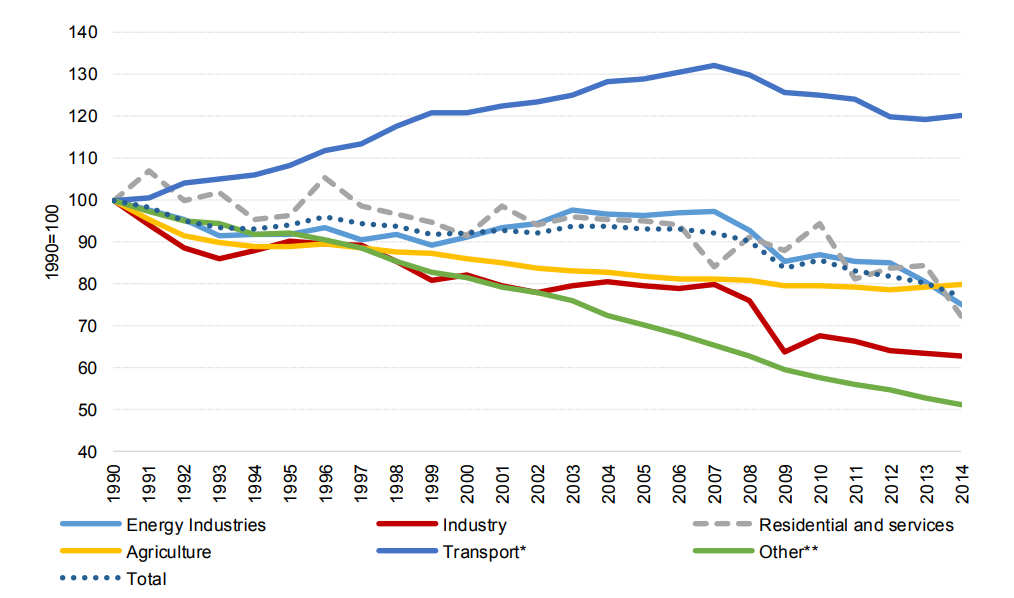
\includegraphics[width=1\textwidth]{4-Emissions-Europe-2016.png}	
		\caption{Evolution of greenhouse gas emissions by sector (1990=100)}{Source: \ac{EEA}}
		\label{fig:4-Emissions-Europe-2016}
	\end{center}
\end{figure}


% http://www.airqualitynow.eu/es/about_indices_definition.php
Some projects like \ac{CITEAIR} has been created by the European Union \cite{citeair} in order to develop efficient means to collect, present and compare air quality data across multiple European cites. One of the results of this project was the craation of the \emph{Air quality now} webpage \cite{airqualitynow}. This page provides a platform to compare real time air quality measurements in different cities of Europe. In this page, air quality is measured in three different time scales: hourly index during the last day, daily index of the previous day and an annual index. Each of this three time scales has 5 indices using a pollution scale that goes from 0 (very low) to 100 (very high). 6 pollutants are measured, these are (PM10, NO2, O3, CO, PM2.5 and SO2). Then, the index is calculated depending on the amount of particles per hour (measured in $\mu g/m^3$), except for CO, in which a 8 hours moving average is used. Figure \ref{fig:4-Pollution-Index-Airqualitynow} shows the relationship between the pollutant measurement and its pollution index assigned.

\begin{figure}[!h]
	\begin{center}
		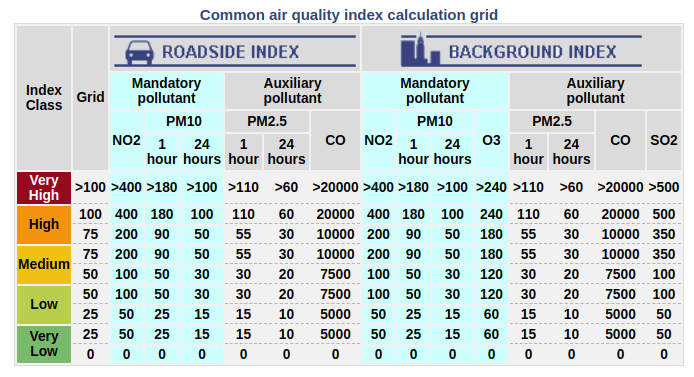
\includegraphics[width=1\textwidth]{4-Pollution-Index-Airqualitynow.png}	
		\caption{Relationship between the pollutant measurement and its pollution index assigned}{Source: Air Quality Now webpage \cite{airqualitynow}}
		\label{fig:4-Pollution-Index-Airqualitynow}
	\end{center}
\end{figure}

% Mencionar ciudades como casos de la problemática.
With the goal of evidencing the problem of traffic pollution in big cities, some examples has been selected. Air quality information about Madrid, Berlin and Paris taken on Tuesday 6th of February 2018 are shown in Figure \ref{fig:4-AirQuality-Details}.
As it can be observed, the pollution indices that day were very high, especially in some cities such as Berlin, where its current roadside pollution level has high (index value between 75 and 100). If the yesterday roadside indices values are compared, it can be shown that in all the selected cities its pollution indices are higher than 50, which means that some measures must be taken, especially in Berlin. This evidence reinforces the fact that some pollution prevention and control mechanisms are necessary.

\begin{figure}[htb]
	\centering
	\subfigure[Madrid]{
		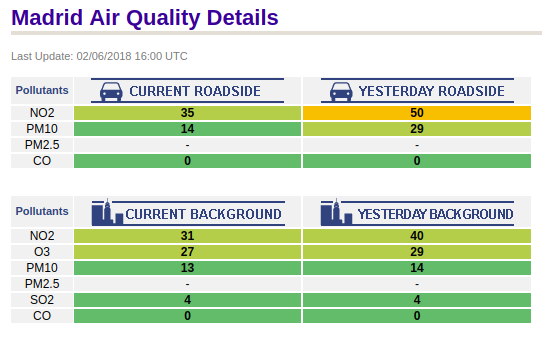
\includegraphics[width=0.74\textwidth]{4-Madrid-AirQuality.png}
		\label{fig:4-Madrid-AirQuality}
	}
	\subfigure[Berlin]{
		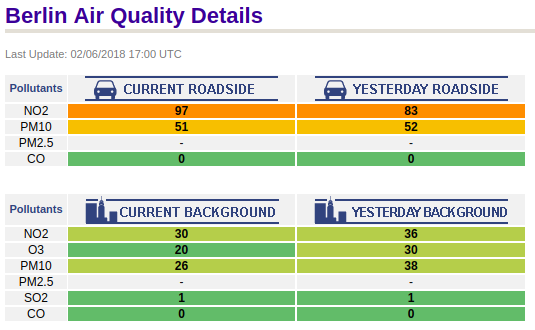
\includegraphics[width=0.74\textwidth]{4-Berlin-AirQuality.png}
		\label{fig:4-Berlin-AirQuality}
	}
	\subfigure[Paris]{
		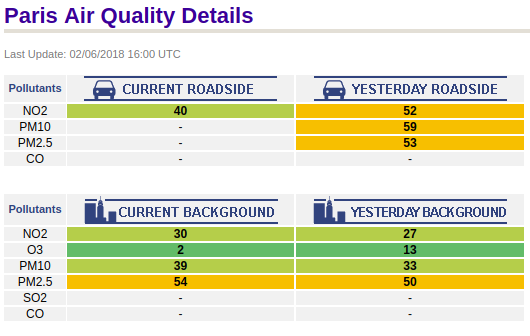
\includegraphics[width=0.74\textwidth]{4-Paris-AirQuality.png}
		\label{fig:4-Paris-AirQuality}
	}
	\caption{Air Quality Details on 6th February 2018 at 18:00}
	\label{fig:4-AirQuality-Details}{Source: Air Quality Now webpage \cite{airqualitynow}}
\end{figure}



\section{Embedded systems}
% Sistemas Empotrados

\subsection{Embedded systems in traffic or environmental surveillance}
% Buscar sistemas embebidos de control de tráfico o medio ambiental.
%	- https://acuraembedded.com/blog/acura-embedded-systems-to-reduce-carbon-emissions-for-public-transport-buses/
%	- ...
% MENCIONAR:
% Estas estaciones solo mide un punto de la ciudad, nosotros buscamos tecnologías baratas y que permitan controlar varios puntos
% Masivo

\section{Raspberry Pi embedded system}
% Raspberry Pi 3 	-> Evolución
%					-> Comparativa con sus competidores
%					->  Raspbian


% ESTO NO:
% Un párrafo hablando de los vectores de movimento y Codificación de vídeo -> H.264/AVC, lincado a los sistemas embebidos 
%	- https://www.raspberrypi.org/blog/vectors-from-coarse-motion-estimation/


